\subsection{Certificate Authority}
\subsubsection{Introduction}
When we talk about a Certificate Authority we talk about a trusted third party that issues Digital Certificates. These certificates are used to digitally sign messages that identifies the sender.\\
We can compare this digital signature with a written signature. The purpose is to guarantee that the sender actually is who it claims to be.\\
But since signatures can be forged, digital signatures offers a number of different encryption algorithms to minimize this risk and offer the client and server a safe way to communicate across the Internet.
\subsubsection{Issuing A Certificate}
Certificate Authorities offers a few ways to verify the validity of an entity when they request a certificate. One way is to do a domain validation - this is the least secure way of verifying that the entity actually is who it claims to be.\\
The second method is to do an extensive validation of the entity, thus ensuring the users that the website really can be trusted.
\subparagraph{Domain Validation}~\\
Like it says above this section, domain validation is the least secure way of validating an entity.\\
This is because the CA (Certicate Authority) only uses the domain to verify an entity. Whatever information they find doing a WHOIS is included in the certificate, and thus trusted by the CA.\\
This means that even though the certificate still uses 128-bit encryption, phishers can obtain a certificate and hide their identity.\\
And if you combine this with a MITM (man-in-the-middle) attack, an attacker can use DNS poisoning and use a domain validated certificate for your domain and redirect users to a fake site, thus enabling the attacker to obtain and collect sensitive user information.
\subparagraph{Extensive Validation}~\\
With an Extensive Validated Certificate you get alot more security for your users. EV Certificates are designed to prevent phishing attacks better than normal domain validated certificates.\\
The extensive validation~\cite{EVCert} checks quite a few different aspects of your organization, including:
\begin{itemize}
	\item Verifying that the organization is registered and active
	\item Verifying that the organization has exclusive rights to use the domain
	\item Verifying that the organization is not on any government blacklists
\end{itemize}
Even though this certificate is more expensive than the normal certificate, it is obvious that it provides many more benefits and that this certificate is the right choice if you really want to ensure the safety for your users.
\begin{wrapfigure}{R}{0.35\textwidth}
	\vspace{-30pt}
  \begin{center}
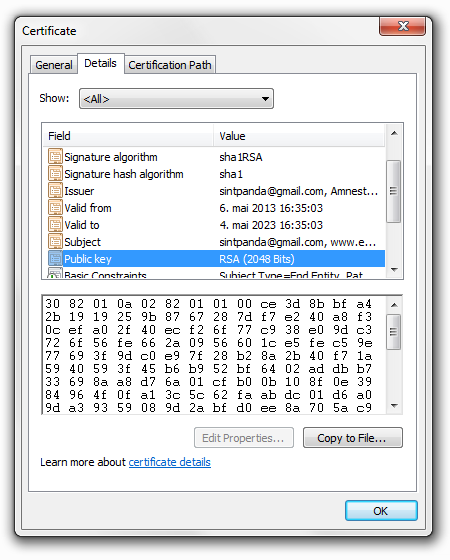
\includegraphics[width=0.40\textwidth]{endusercert}
  \end{center}
	\vspace{-20pt}
  \caption{Client Certificate}
\end{wrapfigure}
\subsubsection{Certificate Structure}

In this section we will briefly go through the structure of an end user certificate and a root certificate.\\
Even though the two certificates does have some fields which are the same, there are a few key differences between them.
\subparagraph{End user certificate}~\\
The end user certificate or, client certificate, basically is the certificate which gets installed on the client's computer.\\
\\
\emph{Version}
\begin{itemize}
	\item This field contains information about the certificate's version. Today there are three versions; 1, 2 \& 3. Higher certificate versions can contain more fields and information.
\end{itemize}
\emph{Serial number}
\begin{itemize}
	\item When the CA issues a certificate, they assign a unique integer to the certificate. This ID has to be unique for each certificate.
\end{itemize}
\emph{Signature algorithm}
\begin{itemize}
	\item Client and servers can communicate using a large range of different encryption algorithms. This field contains the algorithm identifier used by the CA to sign the content using the private key.
\end{itemize}
\emph{Signature hash algorithm}
\begin{itemize}
	\item This field contains information about which hash algorithm to use to hash the content before signing.
\end{itemize}
\emph{Issuer}
\begin{itemize}
	\item In this field we can see information about the entitiy that issued the certificate. For instance; ''C = NO'' means that the issuer is located in Norway (NO) and ''O = Dundergruppen'' is the name of the organization. 
\end{itemize}
\emph{Valid from}
\begin{itemize}
	\item Information about the date the certificate is valid from.
\end{itemize}
\emph{Valid to}
\begin{itemize}
	\item Information about the date the certifiicate is valid to.
\end{itemize}
\emph{Subject}
\begin{itemize}
	\item This field contanins information about the CA that created, issued and signed the certificate.
\end{itemize}
\emph{Public key}
\begin{itemize}
	\item Here we can see the public key and information about the algorithm used.\\
Example:\\
RSA (2048 Bits)\\
''\textit{30 82 01 0a 02 82 01 01 00 ce 3d 8b bf a4 2b 19 19 25 9b 87 67 28 7d f7 e2 40 a8 f3 0c ef a0 2f 40 ec f2 6f 77 c9 38 e0 9d c3 72 6f 56 fe 66 2a 09 56 60 1c e5 fe c5 9e 77 69 3f 9d c0 e9 7f 28 b2 8a 2b 40 f7 1a 59 40 59 3f 45 b6 b9 52 bf 64 02 ad db b7 33 69 8a a8 d7 6a 01 cf b0 0b 10 8f 0e 39 84 96 4f 0f a1 3c 5c 62 fa ab dc 01 d6 a0 9d a3 93 59 08 9d 2a bf d0 ee 8a 70 5a c9 3f 1f 15 b3 36 eb 67 15 e1 8e 5a c5 09 a7 84 bf 31 da a9 07 bf d4 e9 cd 2e 3f a5 e6 03 01 01 d6 67 b2 2b 92 84 06 84 f5 5f e0 d1 d7 5d e8 b0 e9 13 c5 07 db a3 86 5b 73 2f 07 f3 10 aa a4 79 ad e1 00 eb 8d 28 ce 3f ad f5 da 20 a6 f2 36 ef 88 b6 a7 93 9a f4 12 41 ca 99 96 5e 87 31 dd b5 78 d1 2d 83 bd 18 bc ac b2 f9 38 54 68 a3 b9 bb 3d ab 0a a3 6c e1 5c e7 7a d8 10 53 db bb 4d 1c 3d 2e 95 a2 0f 62 d6 ec 53 6f 38 25 02 03 01 00 01}''
\end{itemize}
\emph{Basic Constraints}
\begin{itemize}
	\item If the certificate can be used as a CA it is specified in this field. If not it is specified that the certificate is an ''End Entitiy''.
\end{itemize}
\emph{Key Usage}
\begin{itemize}
	\item Contains information about which operations the public key can be used for.\\
For instance: Digital Signature.
\end{itemize}
\emph{Thumbprint algorithm}
\begin{itemize}
	\item Specifies the algorithm used to hash the certificate.
\\For instance: SHA-1.
\end{itemize}
\emph{Thumbprint}
\begin{itemize}
	\item This is the hash itself. Basically used as an identifier.
\end{itemize}
\subparagraph{Root Certificate}~\\
\begin{wrapfigure}{h}{0.35\textwidth}
	\vspace{-30pt}
  \begin{center}
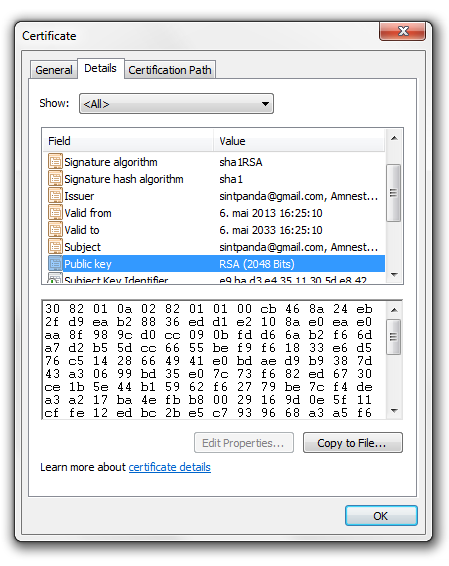
\includegraphics[width=0.40\textwidth]{rootcert}
  \end{center}
	\vspace{-20pt}
  \caption{Root Certificate}
\end{wrapfigure}
Like we mentioned earlier, end user certificates and root certificates contains many of the same fields and values.\\
It is however worth mentioning that the public key is exactly the same in both certificates. This because the client and server use a PKI (Public-key infrastructure)-modell.\\
However, there are differences, and in this section we will go through the field and values that differ between the two certificates.\\\\
\emph{Serial number}
\begin{itemize}
	\item This field contains a unique ID for this root certificate. This is used to distinguish between multiple certificates.
\end{itemize}
\emph{Subject Key Identifier}
\begin{itemize}
	\item This field contains an ID which provides a method of identifying certificates that contain a specific public key. A 160-bit SHA-1 hash of the value of the subjectPublicKey.
\end{itemize}
\emph{Authority Key Identifier}
\begin{itemize}
	\item To help verify the signature on this certificate, this field contains the public key used for that purpose.
\end{itemize}
\emph{Basic Constraints}
\begin{itemize}
	\item Since this is a Root Certificate this field contains the value ''Subject Type=CA''.
\end{itemize}
\subsubsection{Providers}
Worldwide there are a number of certificate authories, and the business is fragmented with national and regional providers.\\
However, certificates used for website security is largely held and issued by a small number of companies, and as of today more than 50 root certificates are trusted in the most popular web browers.\\\\
The market share between the top CA's, from W3Techs survey 2012, shows the following:
\begin{itemize}
	\item{Symantec (including VeriSign, Thawte \& GeoTrust) with 42.9\%}
	\item{Comodo with 26\%}
	\item{GoDaddy with 14\%}
	\item{GlobalSign with 7.7\%}
\end{itemize}

\subsubsection{CA Compromise}
A certificate authority compromise (CA Compromise) is an incident where an attacker is able to use the private key of a CA to issue fake certificates.\\
The worst case scenario is when a Root Certificate Authority is compromised. If that happen the Root Certificate Authority must notify all the relaying parties who trust their certificate, so that the relaying parties can stop trusting that specific certificate.\\\\
If however an Intermediate Root Certificate Authority is compromised, the Root Certificate Authority must revoke those certificates. And obviously the entitiy that got compromised must replace those certificates immediately, since those certificates no longer can be used due to the revocation.

\subparagraph{DigiNotar Incident}~\\
On august 30, 2011, DigiNotar confirmed~\cite{diginotarIncident} that they had been compromised and that Google.com certificates was obtained by the attackers.\\

``\emph{What at first appeared to be a one-off attack targeting Google Gmail users was actually part of a larger breach at Dutch digital certificate authority (CA) DigiNotar, which today confirmed speculation that it indeed was hacked and its SSL and EV-SSL CA system abused by attackers.\\
"The company found out on July 19 that a hacking attempt had happened. At that moment, DigiNotar ordered an external security audit. This audit concluded that all fraudulently issued certificates were revoked. We found out yesterday, through Govcert, that the Google certificate was active. We revoked it immediately," said a spokesman today at Vasco Data Security International, of which the Dutch DigiNotar is a wholly owned subsidiary.}''
% Source: http://www.darkreading.com/attacks-breaches/digital-certificate-authority-hacked-doz/231600498

\subparagraph{Consequences Of A Compromise}~\\ % Følger av en compromise
The CA paradigm is basically a chain-of-trust. So what happens when a CA experience a compromise?\\
If an attacker obtains a certificate for ex. Gmail.com, the attacker can basically impersonate Gmail by issuing forged certificates to its users with the purpose of stealing sensitive information and/or credentials - the trust is then broken.
\\\\
Most operative systems include a feature that will automatically update the system when the developers issues a patch or an update. The common thing is to use certificates to ensure the integrity of the patch, so no malware get's installed on the users system.\\
What happens if an attacker can inpersonate Microsoft and digitally sign his own files using Microsoft's credentials? Well, if an attacker combines that with DNS Poisoning your operative system will see the file issued by the attacker as a legitimate file and install it, thus potensially installing malware on your system.\\
This can obviously be used to steal sensitive information, credentials and/or use the compromised computer in a botnet.